\section{Graph Parsing Algorithm}

We propose a graph parsing algorithm which allows to construct finite representation of parse forest which contains derivation trees for all matched paths in graph.
Finite representation of result set with respect to the specified grammar may be useful not only for results understanding and processing, but also for query debugging. 

Our solution is based on generalized LL (GLL)~\cite{scott2010gll, FastPracticalGLL} parsing algorithm which allows to process arbitrary (including left-recursive and ambiguous) context-free grammars with worst-case cubic time complexity and linear time complexity for LL grammars on a linear input. 

\subsection{Generalized LL Parsing Algorithm}

Classical LL algorithm operates with a pointer to input (position $i$) and with a grammar slot---pointer to grammar in form $N \rightarrow \alpha \cdot x \beta $.
Parsing may be described as a transition of these pointers from the initial position ($i = 0$, $S \rightarrow \cdot \beta $, where $S$ is start nonterminal) to the final ($i = input.Length$, $s \rightarrow \beta \cdot$).
At every step, there are four possible cases in processing of these pointers. 

\begin{enumerate}
\item $N \rightarrow \alpha \cdot x \beta $, when $x$ is a terminal and $x = input[i]$. In this case both pointers should be moved to the right ($i \leftarrow i + 1$, $N \rightarrow \alpha  x \cdot \beta $).
\item $N \rightarrow \alpha \cdot X \beta $, when $X$ is nonterminal. In this case we push return address $N \rightarrow \alpha X \cdot \beta $ to stack and move pointer in grammar to position $X \rightarrow \cdot \gamma$.\label{itm:2}
\item $N \rightarrow \alpha \cdot $. This case means that processing of nonterminal $N$ is finished. We should pop return address from stack and use it as new slot.\label{itm:3}
\item $S \rightarrow \alpha \cdot $, where $S$ is a start nonterminal of grammar. In this case we should report success if $i = input.Length - 1$ or failure otherwise. 
\end{enumerate}

In the second case there can be several slots $X \rightarrow \cdot \gamma$, so a strategy on how to choose one of them to continue parsing is needed.
In LL(k) algorithm lookahead is used, but this strategy is still not good enough because there are context-free languages for which deterministic choice is impossible even for infinite lookahead~\cite{LLnonLL}.
On the contrary to LL(k), generalized LL does not choose at all, handling all possible variants.
Note, that instead of immediate processing of all variants, GLL uses descriptors mechanism to store all possible branches and process them sequentially. 
Descriptor is a quadruple $(L, s, j, a)$ where $L$ is a grammar slot, $s$ is a stack node, $j$ is a position in the input string, and $a$ is a node of derivation tree. 

The stack in parsing process is used to store return information for the parser---a name of function which will be called when current function finishes computation. 
As mentioned before, generalized parsers process all possible derivation branches and parser must store it's own stack for every branch. 
It leads to an infinite stack growth being done naively.  
Tomita-style graph structured stack (GSS)~\cite{Tomita} combines stacks resolving this problem.
Each GSS node contains a pair of position in input and a grammar slot in GLL . 

In order to provide termination and correctness, we should avoid duplication of descriptors, and be able to process GSS nodes in arbitrary order. It is necessary to use the following additional sets for this.
\begin{itemize}
\item $R$---working set which contains descriptors to be processed. Algorithm terminates whenever $R$ is empty.
\item $U$---all created descriptors. Each time when we want to add a new descriptor to $R$, we try to find it in this set first.
This way we process each descriptor only once which guarantee termination of parsing.
\item $P$---popped nodes. Allows to process descriptors (and GSS nodes) in arbitrary order. 
\end{itemize}

Instead of explicit code generation used in classical algorithm, we use table version of GLL~\cite{TableGLL} in order to simplify adaptation to graph processing.
As a result, main control function is different from the original one because it should process LL-like table instead of switching between generated parsing functions.
Control functions of the table based GLL are presented in Algorithm~\ref{mainTblFunctions}.
All other functions are the same as in the original algorithm and their descriptions can be found in the original article~\cite{scott2010gll} or in Appendix~\ref{GLLCode}.

\begin{algorithm}[ht]
\begin{algorithmic}[1]
\caption{Control functions of table version of GLL}
\label{mainTblFunctions}
\Function{dispatcher}{ \ }
  \If{$R.Count \neq 0$}  
      \State{$(L,v,i,cN) \gets R.Get()$}
      \State{$cR \gets dummy$}
      \State{$dispatch \gets false$}
  \Else
      \State{$stop \gets true$}
  \EndIf
\EndFunction

\Function{processing}{ \ }
  \State{$dispatch \gets true$}
  \Switch{$L$}
  \Case{$(X \rightarrow \alpha \cdot x \beta)$ where $x = input[i + 1])$}
       \If{$cN = dummyAST$} 
          \State{$cN \gets \Call{getNodeT}{i}$} 
       \Else 
          \State{$cR \gets \Call{getNodeT}{i}$}
       \EndIf
       \State{$i \gets i + 1$}
       \State{$L \gets (X \rightarrow \alpha x \cdot \beta)$}
       \If{$cR \neq dummy$}
          \State{$cN \gets \Call{getNodeP}{L, cN, cR}$} 
       \EndIf
       \State{$dispatch \gets false$}        
  \EndCase
  \Case{$(X \rightarrow \alpha \cdot x \beta)$ where $x$ is nonterminal}
       \State{$v \gets$ \Call{create}{$(X \rightarrow \alpha x \cdot \beta), v, i, cN$}}
       \State{$slots \gets pTable[x][input[i]]$}
       \ForAll{$L \in slots$}
          \State{\Call{add}{$L,v,i,dummy$}} 
       \EndFor
  \EndCase
  \Case{$(X \rightarrow \alpha \cdot )$}
       \State{\Call{pop}{v,i,cN}} 
  \EndCase
  \Case{$(S \rightarrow \alpha \cdot )$ when $S$ is start nonterminal}
       \State{final result processing and error notification} 
  \EndCase
  \EndSwitch
\EndFunction

\Function{control}{}
  \While{not $stop$}  
      \If{$dispatch$}
        \State{\Call{dispatcher}{ \ }}
      \Else
         \State{\Call{processing}{ \ }}
      \EndIf
  \EndWhile
\EndFunction

\end{algorithmic}
\end{algorithm}

There can be more than one derivation tree of a string with relation to ambiguous grammar.
Generalized LL build all such trees and compact them in a special data structure Shared Packed Parse Forest~\cite{SPPF}, which will be described in the following section.

\subsection{Shared Packed Parse Forest}

Binarized Shared Packed Parse Forest (SPPF)~\cite{brnglr} compresses derivation trees optimally reusing common nodes and subtrees.
Version of GLL which uses this structure for parsing forest representation achieves worst-case cubic space complexity~\cite{gllParsingTree}.

Let us present an example of SPPF for the input sentence \verb|"ababab"| and ambiguous grammar $G_0$ (fig~\ref{grammarG0}).

\begin{figure}[h]
   \begin{center}
   \[
\begin{array}{rl}

   0: & S \rightarrow \varepsilon  \\
   1: & S \rightarrow a \ S \ b \\
   2: & S \rightarrow S \ S    
\end{array}
\]
   \caption{Grammar $G_0$}
   \label{grammarG0}        
   \end{center}
\end{figure}


There are two different leftmost derivations of the given sentence w.r.t. grammar $G_0$, hence SPPF contains two different derivation trees. Resulting SPPF(fig.~\ref{sppf}) and two trees extracted from it (fig.~\ref{tree1} and fig.~\ref{tree2}) are presented in the figure~\ref{sppfSample}. 
 
\begin{figure*}[ht]
    \begin{center}
    \centering
    \begin{subfigure}[b]{0.3\textwidth}
        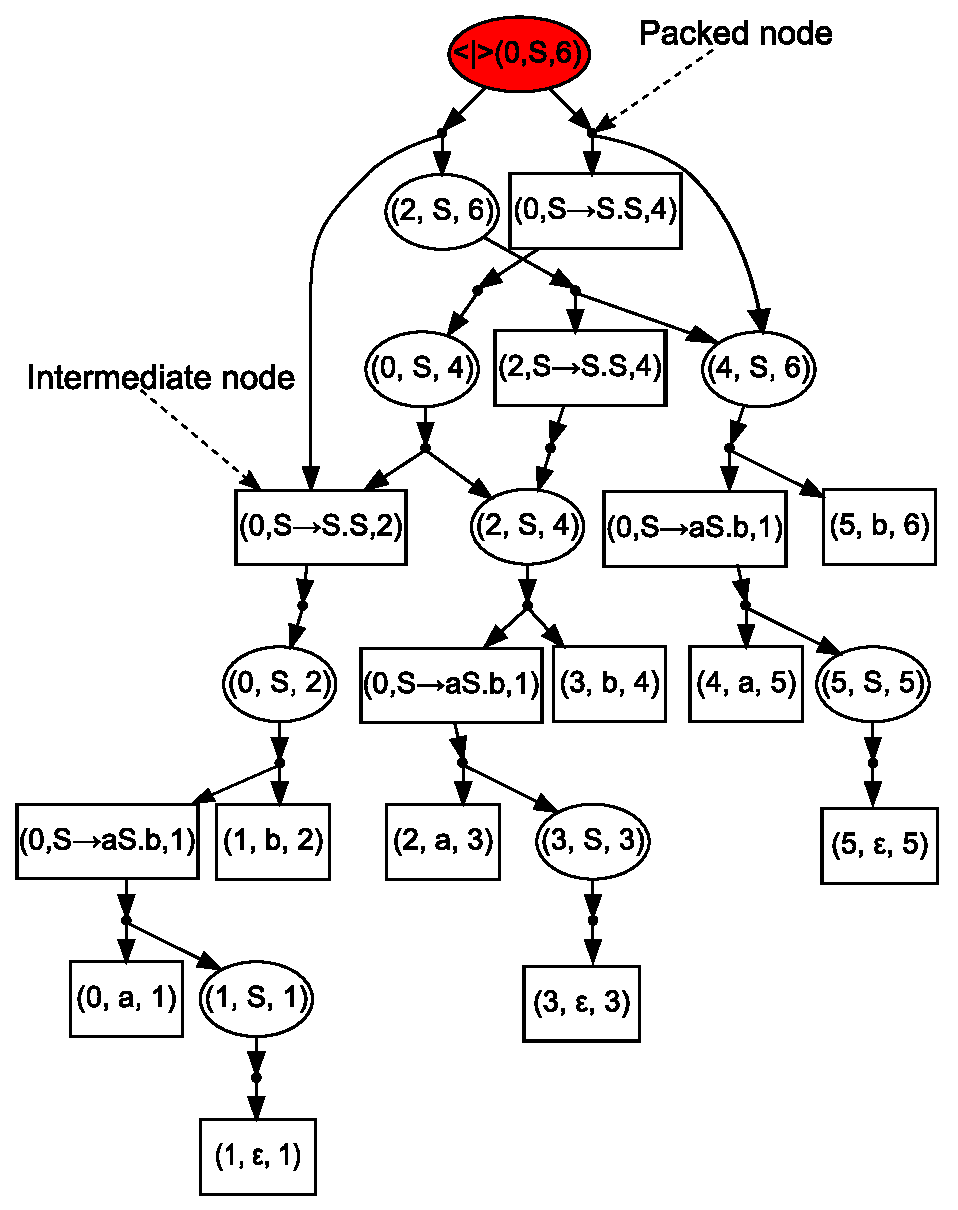
\includegraphics[width=\textwidth]{dot/Brackets.pdf}
        \caption{SPPF}
        \label{sppf}        
    \end{subfigure}
    ~
    \begin{subfigure}[b]{0.3\textwidth}
        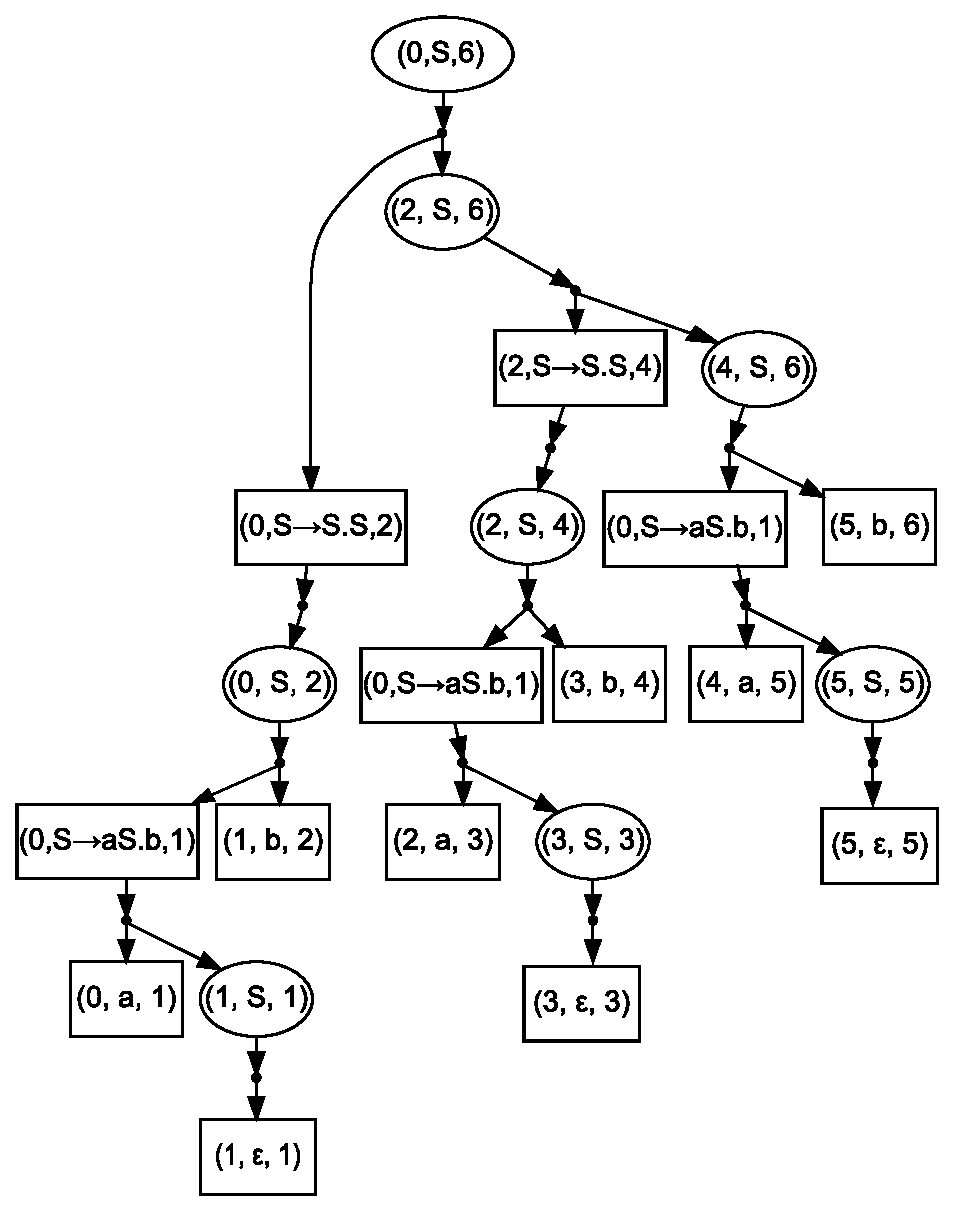
\includegraphics[width=\textwidth]{dot/Brackets1.pdf}
        \caption{First derivation tree}
        \label{tree1}        
    \end{subfigure}
    ~
    \begin{subfigure}[b]{0.3\textwidth}
        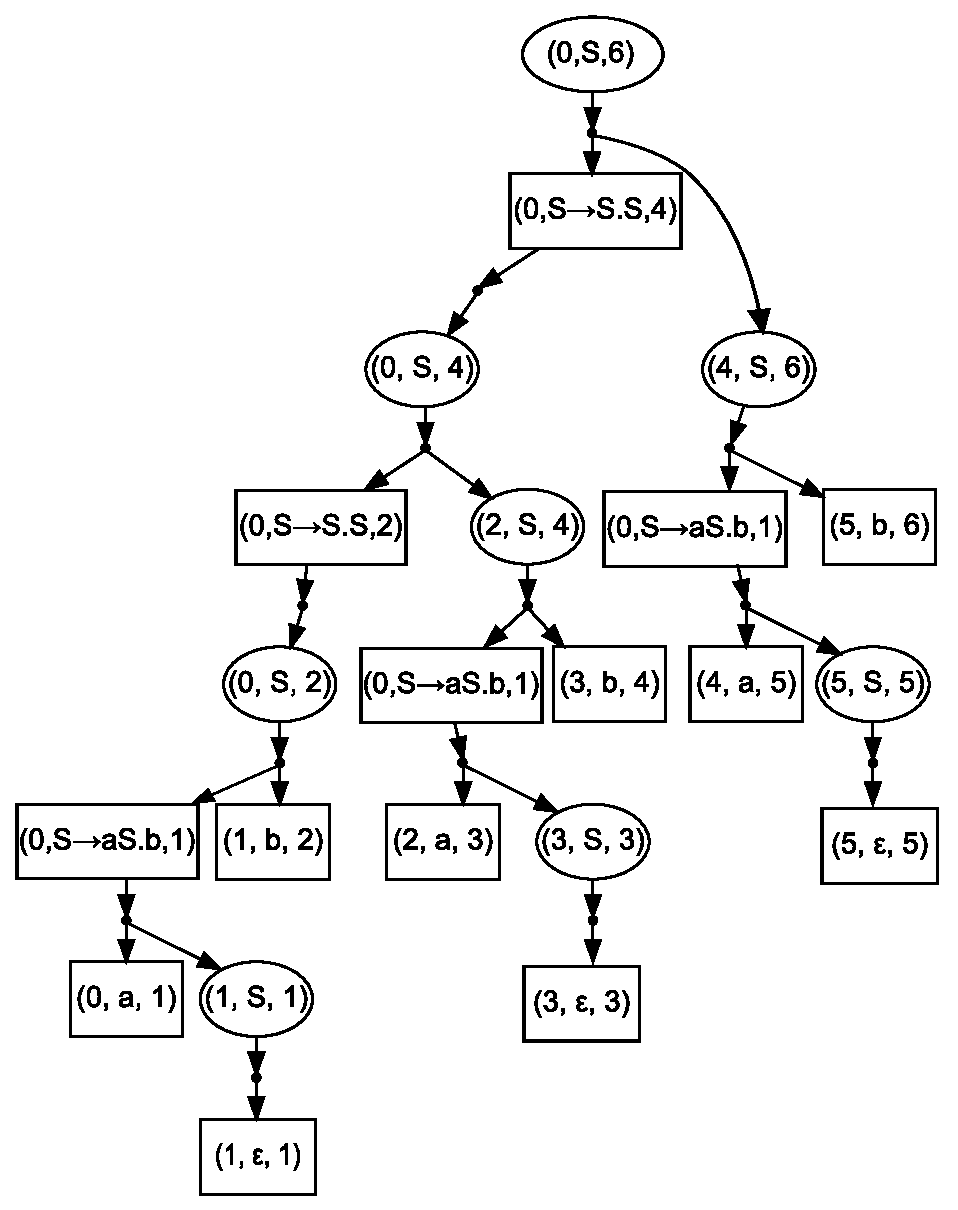
\includegraphics[width=\textwidth]{dot/Brackets2.pdf}
        \caption{Second derivation tree}
        \label{tree2}        
    \end{subfigure}
    \caption{SPPF for sentence \textbf{\texttt{"ababab"}} and grammar $G_0$}
    \label{sppfSample}
    \end{center}                
\end{figure*}

Binarized SPPF can be represented as a graph in which each node has one of four types described below with correspondent graphical notation.
Let $i$ and $j$ be the start and the end positions of substring, and let us call a tuple $(i,j)$ an \textit{extension} of node.

\begin{itemize}
    \item Node of rectangle shape labeled with $(i, T, j)$ is a terminal node.     
    \item Node of oval shape labeled with $(i, N, j)$ is a nonterminal node. 
    This node denotes that there is at least one derivation for substring $\alpha=\omega[i..j-1]$ such that $N \Rightarrow^*_G \alpha, \alpha = \omega[i..j-1] $.
    All derivation trees for the given substring and nonterminal can be extracted from SPPF by left-to-right top-down graph traversal started from respective node. 
    We use filled shape and label of form $(<\mkern-11mu | \mkern-11mu> (i, N, j))$ to denote that there are multiple derivations from nonterminal $N$ for substring $\omega[i..j-1]$.
    \item Node of rectangle shape labeled with $(i,t,j)$, where $t$ is a grammar slot, is an intermediate node: a special kind of node used for binarization of SPPF.
    \item Packed node labeled with $(N \rightarrow \alpha \cdot \beta, k)$. In our pictures, we use dot shape for these nodes and omit labels because they are important only on SPPF constriction stage.
    Subgraph with ``root'' in such node is one variant of derivation from nonterminal $N$ in case when the parent is a nonterminal node labeled with $(<\mkern-9mu | \mkern-9mu> (i, N, j))$.

\end{itemize}

In our examples we remove redundant intermediate and packed nodes from the SPPF to simplify it and to decrease the size of structure.

\subsection{GLL-based Graph Parsing}

In this section we present such modification of GLL algorithm, that for input graph $M$, set of start vertices $V_s\subseteq V$, set of final vertices $V_f\subseteq V$, and grammar $G_1$, it returns SPPF which contains all derivation trees for all paths $p$ in $M$, such that $\Omega(p) \in L(G_1)$, and $p.start \in V_s,\ p.end \in V_f$.
In other words, we propose GLL-based algorithm which can solve language constrained path problem.

First of all, notice that an input string for classical parser can be represented as a linear graph, and positions in the input are vertices of this graph.
This observation can be generalized to arbitrary graph with remark that for a position there is a set of labels of all outgoing edges for given vertex instead of just one next symbol. 
Thus, in order to use GLL for graph parsing we need to use graph vertices as positions in input and modify \textbf{Processing} function to process multiple ``next symbols''.
Required modifications are presented in the Algorithm~\ref{modifAlgo}~(line \textbf{5} and \textbf{17}).
Small modification is also required for initialization of $R$ set: it is necessary to add not only one initial descriptor but the set of descriptors for all vertices in $V_s$.
All other functions are reused from original algorithm without any changes.

\begin{algorithm}[ht]
\begin{algorithmic}[1]
\caption{\textbf{Processing} function modified in order to process arbitrary directed graph}
\label{modifAlgo}
\Function{processing}{\ }
  \State{$dispatch \gets true$}
  \Switch{$L$}
  \Case{$(X \rightarrow \alpha \cdot x \beta)$ where $x$ is terminal}
       \boldnext
       \ForAll{$\{ e | e \in input.outEdges(i), tag(e) = x \}$}
       \State{$new\_cN \gets cN$}
       \If{$new\_cN = dummyAST$} 
          \State{$new\_cN \gets \Call{getNodeT}{e}$} 
       \Else 
          \State{$new\_cR \gets \Call{getNodeT}{e}$}
       \EndIf
       \State{$L \gets (X \rightarrow \alpha x \cdot \beta)$}
       \If{$new\_cR \neq dummy$}
          \State{$new\_cN \gets \Call{getNodeP}{L, new\_cN, new\_cR}$} 
       \EndIf
       \State{\Call{add}{$L,v,target(e),new\_cN$}}
       \EndFor
  \EndCase
  \Case{$(X \rightarrow \alpha \cdot x \beta)$ where $x$ is nonterminal}
       \State{$v \gets$ \Call{create}{$(X \rightarrow \alpha x \cdot \beta), v, i, cN$}}
       \boldnext
       \State{$slots \gets \bigcup_{e \in input.OutEdges(i)} pTable[x][e.Token]$}
       \ForAll{$L \in slots$}
          \State{\Call{add}{$L,v,i,dummy$}} 
       \EndFor
  \EndCase
  \Case{$(X \rightarrow \alpha \cdot )$}
       \State{\Call{pop}{$v,i,cN$}} 
  \EndCase
  \Case{$\_$}
       \State{final result processing and error notification} 
  \EndCase
  \EndSwitch
\EndFunction

\end{algorithmic}
\end{algorithm}

Note that our solution handles arbitrary numbers of start and final vertices, which allows one to solve different kinds of problems arising in the field, namely all paths in graph, all paths from specified vertex, all paths between specified vertices. 
Also SPPF represents a structure of paths in terms of grammar which provides exhaustive information about result. 

Note that termination of proposed algorithm is inherited from the basic GLL algorithm.
We process finite graphs, hence the set of positions is finite, and tree construction has not been changed. 
As a result, the total number of descriptors is finite, and each of them is added in $R$ only once, thus main loop is finite.
